\documentclass[tikz]{standalone}
%\usepackage{tikz}
\usetikzlibrary{matrix,arrows,positioning,backgrounds}
\usetikzlibrary{decorations.pathmorphing,decorations.pathreplacing}
\begin{document}
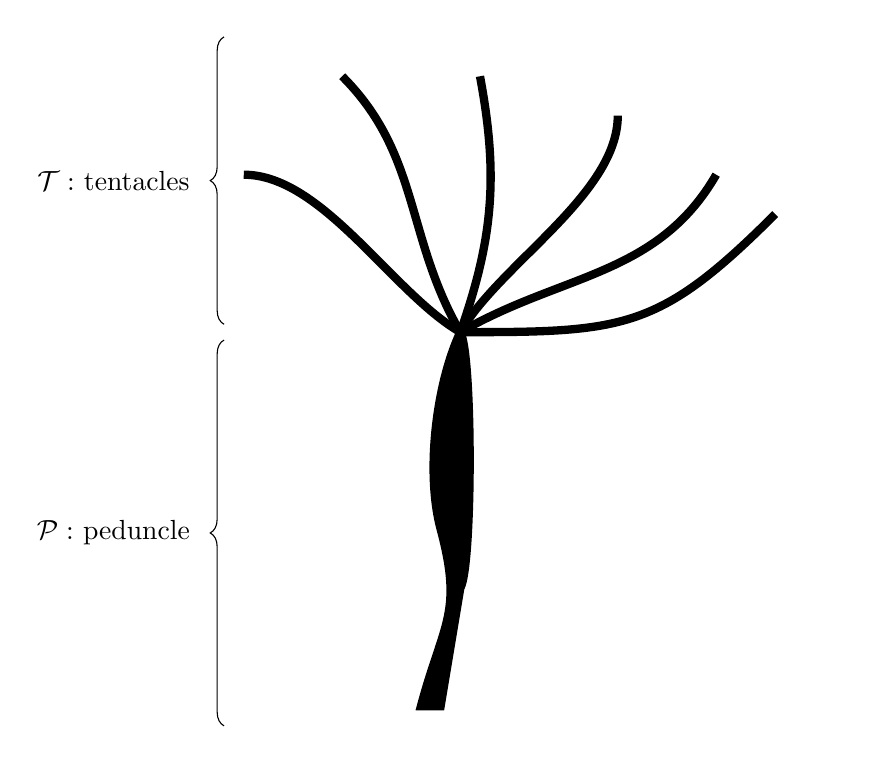
\begin{tikzpicture}
\tikzstyle{tan}=[draw=black, line width=3pt]
\tikzstyle{pen}=[fill=black, line width=3pt]
\node  (0) at (-0.25, -0.5) {};
\node  (2) at (-0.5, -2.75) {};
\node  (4) at (-1.5, 5.25) {};
\node  (5) at (2, 4.75) {};
\node  (6) at (-2.75, 4) {};
\node  (7) at (4, 3.5) {};
\node  (8) at (3.25, 4) {};
\node  (9) at (0, 2) {};
\node  (10) at (0.25, 5.25) {};
\node  (11) at (-0.25, -2.75) {};
\node  (12) at (0, -1.25) {};
\node  (13) at (-3, 5.75) {};
\node  (15) at (-3, 2.1) {};
\node  (16) at (-3, 1.9) {};
\node  (17) at (-3, -3) {};
\node  (18) at (5, -3) {};
\node  (19) at (5, -2.5) {};
\node  (20) at (5, -2.4) {};
\node  (21) at (5, 5.75) {};
\draw [style=tan, in=0, out=150, looseness=0.75] (9.center) to (6.center);
\draw [style=tan, in=120, out=-45] (4.center) to (9.center);
\draw [style=tan, in=30, out=-120] (8.center) to (9.center);
\draw [style=tan, in=60, out=-90, looseness=0.75] (5.center) to (9.center);
\draw [style=tan, in=0, out=-135, looseness=1.25] (7.center) to (9.center);
\draw [style=tan, bend left=15] (10.center) to (9.center);
\draw [style=pen] (2.center)
to (11.center)
to (12.center)
to [bend right, looseness=0.25] (9.center)
to [in=105, out=-115, looseness=0.75] (0.center)
to [in=75, out=-75, looseness=1.25] cycle;
\draw [decorate,decoration={brace,amplitude=5pt}] (15.center) --
(13.center) node [black,midway,xshift=-4em] {$\mathcal{T}:$ tentacles};
\draw [decorate,decoration={brace,amplitude=5pt}]
(17.center) -- (16.center) node [black,midway,xshift=-4em] {$\mathcal{P}:$ peduncle};
% \draw [decorate,decoration={brace,amplitude=5pt}]  (19.center) -- (18.center)
%  node [black,midway,xshift=4em] {$\mathcal{D}:$ basal disk};
% \draw [decorate,decoration={brace,amplitude=5pt}]  (21.center) -- (20.center)
%  node [black,midway,xshift=4em] {$\mathcal{B}:$ body};
\end{tikzpicture}
\end{document}
